\ifx\PREAMBLE\undefined
\documentclass{report}
\usepackage[format = hang, font = bf]{caption}
% The following is needed in order to make the code compatible
% with both latex/dvips and pdflatex. Added for using UML generated by MetaUML.
\ifx\pdftexversion\undefined
\usepackage[dvips]{graphicx}
\else
\usepackage[pdftex]{graphicx}
\DeclareGraphicsRule{*}{mps}{*}{}
\fi
\usepackage{array}
\usepackage{amsmath}
\usepackage{amsthm}
\usepackage{mathtools}
\usepackage{boxedminipage}
\usepackage{listings}
\usepackage{makecell}%diagonal line in table
\usepackage{float}%allowing forceful figure[H]
\usepackage{xcolor}
\usepackage{amsfonts}%allowing \mathbb{R}
\usepackage{amssymb}
\usepackage{alltt}
\usepackage{algorithmicx}
\usepackage[chapter]{algorithm} 
%chapter option ensures that algorithms are numbered within each chapter rather than in the whole article
\usepackage[noend]{algpseudocode} %If end if, end procdeure, etc is expected to appear, remove the noend option
\usepackage{xspace}
\usepackage{color}
\usepackage{url}
\def\UrlBreaks{\do\A\do\B\do\C\do\D\do\E\do\F\do\G\do\H\do\I\do\J\do\K\do\L\do\M\do\N\do\O\do\P\do\Q\do\R\do\S\do\T\do\U\do\V\do\W\do\X\do\Y\do\Z\do\[\do\\\do\]\do\^\do\_\do\`\do\a\do\b\do\c\do\d\do\e\do\f\do\g\do\h\do\i\do\j\do\k\do\l\do\m\do\n\do\o\do\p\do\q\do\r\do\s\do\t\do\u\do\v\do\w\do\x\do\y\do\z\do\0\do\1\do\2\do\3\do\4\do\5\do\6\do\7\do\8\do\9\do\.\do\@\do\\\do\/\do\!\do\_\do\|\do\;\do\>\do\]\do\)\do\,\do\?\do\'\do+\do\=\do\#\do\-}
\usepackage[breaklinks = true]{hyperref}
\lstset{
language = C++, 
showspaces = false,
breaklines = true, 
tabsize = 2, 
numbers = left, 
extendedchars = false, 
basicstyle = {\ttfamily \footnotesize}, 
keywordstyle=\color{blue!70}, 
commentstyle=\color{gray}, 
frame=shadowbox, 
rulesepcolor=\color{red!20!green!20!blue!20}, 
numberstyle={\color[RGB]{0,192,192}}, 
moredelim=[is][\underbar]{_}{_}
}
\mathchardef\myhyphen="2D
% switch-case environment definitions
\algblock{switch}{endswitch} 
\algblock{case}{endcase}
%\algrenewtext{endswitch}{\textbf{end switch}} %If end switch is expected to appear, uncomment this line.
\algtext*{endswitch} % Make end switch disappear
\algtext*{endcase}
\algnewcommand\algorithmicinput{\textbf{input:}}
\algnewcommand\Input{\item[\algorithmicinput]}
\algnewcommand\algorithmicoutput{\textbf{output:}}
\algnewcommand\Output{\item[\algorithmicoutput]}
\allowdisplaybreaks
\newtheorem{theorem}{Theorem}[chapter]
\newtheorem{corollary}[theorem]{Corollary}
\newtheorem{lemma}[theorem]{Lemma}
\newtheorem{definition}{Definition}[chapter]
\begin{document}
\fi
\chapter{Divide and Conquer Algorithms}
A typical divide-and-conquer solution to a problem consists of the following steps:
\begin{enumerate}
\item Divide the problem into smaller sub-problems.
\item Conquer the sub-problems via recursive calls.
\item Combine solutions of sub-problems into a solution to the original problem, often involving some clean-up work.
\end{enumerate}
\section{Inversion Counting Problem}
We will solve the inversion problem using the divide-and-conquer paradigm. The problem is described as follow.
\begin{description}
\item[Input]An array $A$ containing numbers $1,2,\dots,n$ in some arbitrary order.
\item[Output]Number of inversions in this array, i.e. number of pairs $[i,j]$ such that $i<j$ and $A[i]>A[j]$.
\end{description}
A geometrical solution to the problem is to draw two parallel series of points, mark one series in the order inside array $A$, and mark the other in the order $1,2,\dots,n$. Connect points marked by the same number, i.e. 1 with 1, 2 with 2, etc, then the number of crossing lines is exactly the number of inversions. 

The inversion number is widely useful in comparison and recommendation systems. A movie rating website wants to compare tastes of its users and recommend to a user movies liked by other users with similar taste to his. One criterion of such comparison is to pick the ratings given by one user to a series of movies and compare them against other users' ratings by calculating the number of inversions. The fewer inversions there are, the more similar their tastes are.

A brute-force approach is obviously $\Theta(n^2)$. We can do better by applying the divide-and-conquer paradigm. Suppose that the array has been divided into two halves. An inversion $[i,j]$ is called a left inversion if both $i,j$ are in the left half, a right inversion if they are both in the right half, and a split inversion if $i$ is in the left half and $j$ is in the right half. A high-level divide-and-conquer algorithm is provided in Algorithm \ref{inversioncounting}. If \texttt{countSplitInv} can be implemented as $\Theta(n)$, then the whole algorithm will be $\Theta(n\log n)$.
\begin{algorithm}[ht]
\caption{Divide-and-conquer Inversion Counting}\label{inversioncounting}
\begin{algorithmic}[1]
\Input\Statex{Array A}
\Output\Statex{Number of inversions in A}
\Function{count}{Array A}
\If{A.len == 1}\State{return 0}
\Else
\State{x = count(1st half of A)}\Comment{Left inversions.}
\State{y = count(2nd half of A)}\Comment{Right inversions.}
\State{z = countSplitInv(A)}\Comment{Count split inversions.}
\State{return x+y+z}
\EndIf
\EndFunction
\end{algorithmic}
\end{algorithm}

The implementation of \texttt{countSplitInv} seems quite subtle, but it can actually be developed from merge sort. In Algorithm \ref{inversioncounting}, the subroutine \texttt{count} only counts the number of inversions. In addition to that, we rename it with \texttt{sortAndCount} and require that it also sorts the array. Subroutine \texttt{countSplitInv} now becomes \texttt{mergeAndCountSplitInv}. It merges the two sorted sub-arrays into one sorted array and counts the number of split inversions.

If there exists no split inversion, it must be the case that any element of the left sub-array A is smaller than any element of the right sub-array B. As a result, when merging the two sorted sub-arrays, A will be exhausted before any element of B is put in the result. Once an element of B is chosen during the merging process before A is exhausted, every element left in A forms an inversion with it. Algorithm \ref{countsplitinversion}, developed from Algorithm \ref{mergehalves}%in file Introduction.tex
, uses this idea to carry out the \texttt{mergeAndCountSplitInv} process. It is still $\Theta(n)$, thus our inversion counting algorithm is guaranteed to be $\Theta(n\log n)$.
\begin{algorithm}[ht]
\caption{Merge and Count Split Inversion}\label{countsplitinversion}
\begin{algorithmic}[1]
\Input
\Statex{A = 1st sorted sub-array, of length $\lfloor n/2 \rfloor$}
\Statex{B = 2nd sorted sub-array, of length $\lceil n/2 \rceil$}
\Output
\Statex{C = sorted array of length $n$}
\Statex{numSplitInv = number of split inversions}
\State{i = 1, j = 1, numSplitInv = 0}
\For{k = 1 \textbf{to} $n$}
\If{i $>$ A.len}\Comment{A has been exhausted}
\State{C[k] = B[j++]}
\ElsIf{j $>$ B.len}\Comment{B has been exhausted}
\State{C[k] = A[i++]}
\ElsIf{A[i] $\leq$ B[j]}\Comment{In this case equality is actually impossible.}
\State{C[k] = A[i++]}
\Else\Comment{A[i]$>$B[j]}
\State{C[k] = B[j++]}
\State{numSplitInv += A.len}
\EndIf
\EndFor
\end{algorithmic}
\end{algorithm}
\section{Matrix Multiplication}
Matrix multiplication is an important mathematical problem.
\begin{description}
\item[Input]Two matrices $X,Y$ of dimension $N\times N$.
\item[Output]Product matrix $Z=X\cdot Y$.
\end{description}
The definition of matrix multiplication is $Z_{ij}=\sum\limits_{k=1}^NX_{ik}Y_{kj}$. Calculating the product matrix directly will result in a $\Theta(n^3)$ algorithm.\footnote{Here the input size is $\Theta(n^2)$, rather than $\Theta(n)$.} We will introduce an ingenious divide-and-conquer algorithm developed by Strassen that is more efficient.

At first sight, it might seem plausible to divide each matrix into 4 sub-matrices of dimension $N/2\times N/2$ in the divide phase of the divide-and conquer process:
\begin{equation*}
XY=\begin{pmatrix}A&B\\C&D\end{pmatrix}\begin{pmatrix}E&F\\G&H\end{pmatrix}=
\begin{pmatrix}
AE+BG&AF+BH\\CE+DG&CF+DH
\end{pmatrix}.
\end{equation*}
However, this division does not make great difference. The algorithm is still $\Theta(n^3)$, as we will prove later. Recall that in the Karatsuba Multiplication algorithm, we reduced the number of products by 1 by applying the Gauss's trick: obtain some products by linear combination of other products, rather than direct multiplication. Since addition/subtraction is generally more efficient than multiplication, it usually pays off to appropriately choose the products to calculate in order to reduce the number of products to calculate. In the naive divide-and-conquer design above, we have to calculate 8 products of sub-matrices. Strassen's brilliant algorithm reduces this number to 7, as shown in Algorithm \ref{strassen}, and ends up with smaller time consumption. 
\begin{algorithm}
\caption{Strassen's Matrix Multiplication}\label{strassen}
\begin{algorithmic}[1]
\Input\Statex{Two matrices $X,Y$ of dimension $N\times N$}
\Output\Statex{Matrix product $X\cdot Y$}
\State{Divide the matrices: $X=\begin{pmatrix}A&B\\C&D\end{pmatrix}$, $Y=\begin{pmatrix}E&F\\G&H\end{pmatrix}$}
\State{Recursively calculate
\begin{align*}
P_1&=A(F-H),\:P_2=(A+B)H,\:P_3=(C+D)E,\:P_4=D(G-E)\\
P_5&=(A+D)(E+H),\:P_6=(B-D)(G+H),\:P_7=(A-C)(E+F)\\
\end{align*}}
\State{Linearly combine the products in step 2 to obtain $XY$:
\begin{equation*}
XY=\begin{pmatrix}
P_5+P_4-P_2+P_6&P_1+P_2\\
P_3+P_4&P_1+P_5-P_3-P_7\\
\end{pmatrix}=\begin{pmatrix}
AE+BG&AF+BH\\CE+DG&CF+DH
\end{pmatrix}\end{equation*}}
\end{algorithmic}
\end{algorithm}
The explanation of its time complexity, as well as that of the naive divide-and-conquer algorithm will be addressed later. 
\section{Closest Pair}
The closest pair problem is the first computational geometry problem we meet. 
\begin{description}
\item[Input]A set of $n$ points $P=\{p_1,\dots,p_n\}$ on the $\mathbb{R}^2$ plane. For simplicity, we assume that they have distinct $x$ coordinates and $y$ coordinates.
\item[Output]A pair of distinct points $p^*,q^*\in P$ that minimizes the Euclidean distance between two points $d(p,q)$ with $p,q\in P$.
\end{description}
A brute-force algorithm is obviously $\Theta(n^2)$. A divide-and-conquer approach can improve it to $\Theta(n\log n)$. Its subtlety lies, as usual, in the 3rd step: combination of solutions to the sub-problems. As preparation before the divide-and-conquer, we sort the points respectively by $x$ and $y$ coordinates, and note the results as $P_x,P_y$. The sort process is $\Theta(n\log n)$ using merge sort, thus we can obtain a $\Theta(n \log n)$ algorithm as long as the divide-and-conquer process takes no more than $\Theta(n\log n)$. 

The skeleton of the process is shown in Algorithm \ref{closetpair}. \texttt{ClosestSplitPair} remains to be illustrated. It outputs the ``split pair'', i.e. one point in $Q$ and the other in $R$, with minimum distance.
\begin{algorithm}[ht]
\caption{Closest Pair Searching ClosetPair($P_x,P_y$)}\label{closetpair}
\begin{algorithmic}[1]
\Input\Statex{A set of $n$ points $P=\{p_1,\dots,p_n\}$ on $\mathbb{R}^2$, sorted respectively by $x$ and $y$ coordinates as $P_x$ and $P_y$}
\Output\Statex{$p,q$ with minimum Euclidean distance}
\State{Let $Q$ be the left half of $P$ and $R$ be right half of $P$. According to $P_x,P_y$, form $Q_x,Q_y,R_x,R_y$, i.e. $Q,R$ sorted by $x$ and $y$ coordinates.}\Comment{$\Theta(n)$}
\State{$(p_1,q_1)$ = ClosestPair($Q_x,Q_y$)}
\State{$(p_2,q_2)$ = ClosestPair($R_x,R_y$)}
\State{$\delta=\min\{d(p_1,q_1),d(p_2,q_2)\}$}
\State{$(p_3,q_3)$ = ClosetSplitPair($P_x,P_y,\delta$)}\Comment{Should be $O(n)$}
\State{Return the best among $(p_1,q_1),(p_2,q_2)$ and $(p_3,q_3)$}
\end{algorithmic}
\end{algorithm}

Let $\overline{x}$ represent the largest $x$ coordinate in $Q$, i.e. in the left half of $P$. Since we have $P_x$, $\overline{x}$ can be obtained in $O(1)$ time. Define $S_y$ as points in $P$ with $x$ coordinate inside $[\overline{x}-\delta,\overline{x}+\delta]$, sorted by $y$ coordinate. We have the following lemma.
\begin{lemma}\label{lemmaforclosesplitpair}
Let $p\in Q,q\in R$ be the split pair with $d(p,q)<\delta$. Then we must have
\begin{itemize}
\item $p,q\in S_y$;
\item $p,q$ are at most 7 positions away from each other in $S_y$. 
\end{itemize}
\end{lemma}
\begin{proof}
Let $p(x_1,y_1)\in Q$, $q(x_2,y_2)\in R$, and we have 
$$d(p,q)=\sqrt{(x_1-x_2)^2+(y_1-y_2)^2}<\delta.$$
Since $\overline{x}$ is the largest coordinate in $Q$, we have 
$$x_1\leq \overline{x}\leq x_2.$$
Thus 
\begin{align*}
\lvert x_2-\overline{x}\rvert=x_2-\overline{x}\leq x_2-x_1\leq\sqrt{(x_1-x_2)^2+(y_1-y_2)^2}<\delta,\\
\lvert x_1-\overline{x}\rvert=\overline{x}-x_1\leq x_2-x_1\leq\sqrt{(x_1-x_2)^2+(y_1-y_2)^2}<\delta.
\end{align*}
Which leads to the conclusion
$$x_1,x_2\in[\overline{x}-\delta,\overline{x}+\delta].$$
This can be directly translated to the first claim of the lemma: $p,q\in S_y$. Figure \ref{pq7position} helps to prove the 2nd claim.  
\begin{figure}[H]
\centering
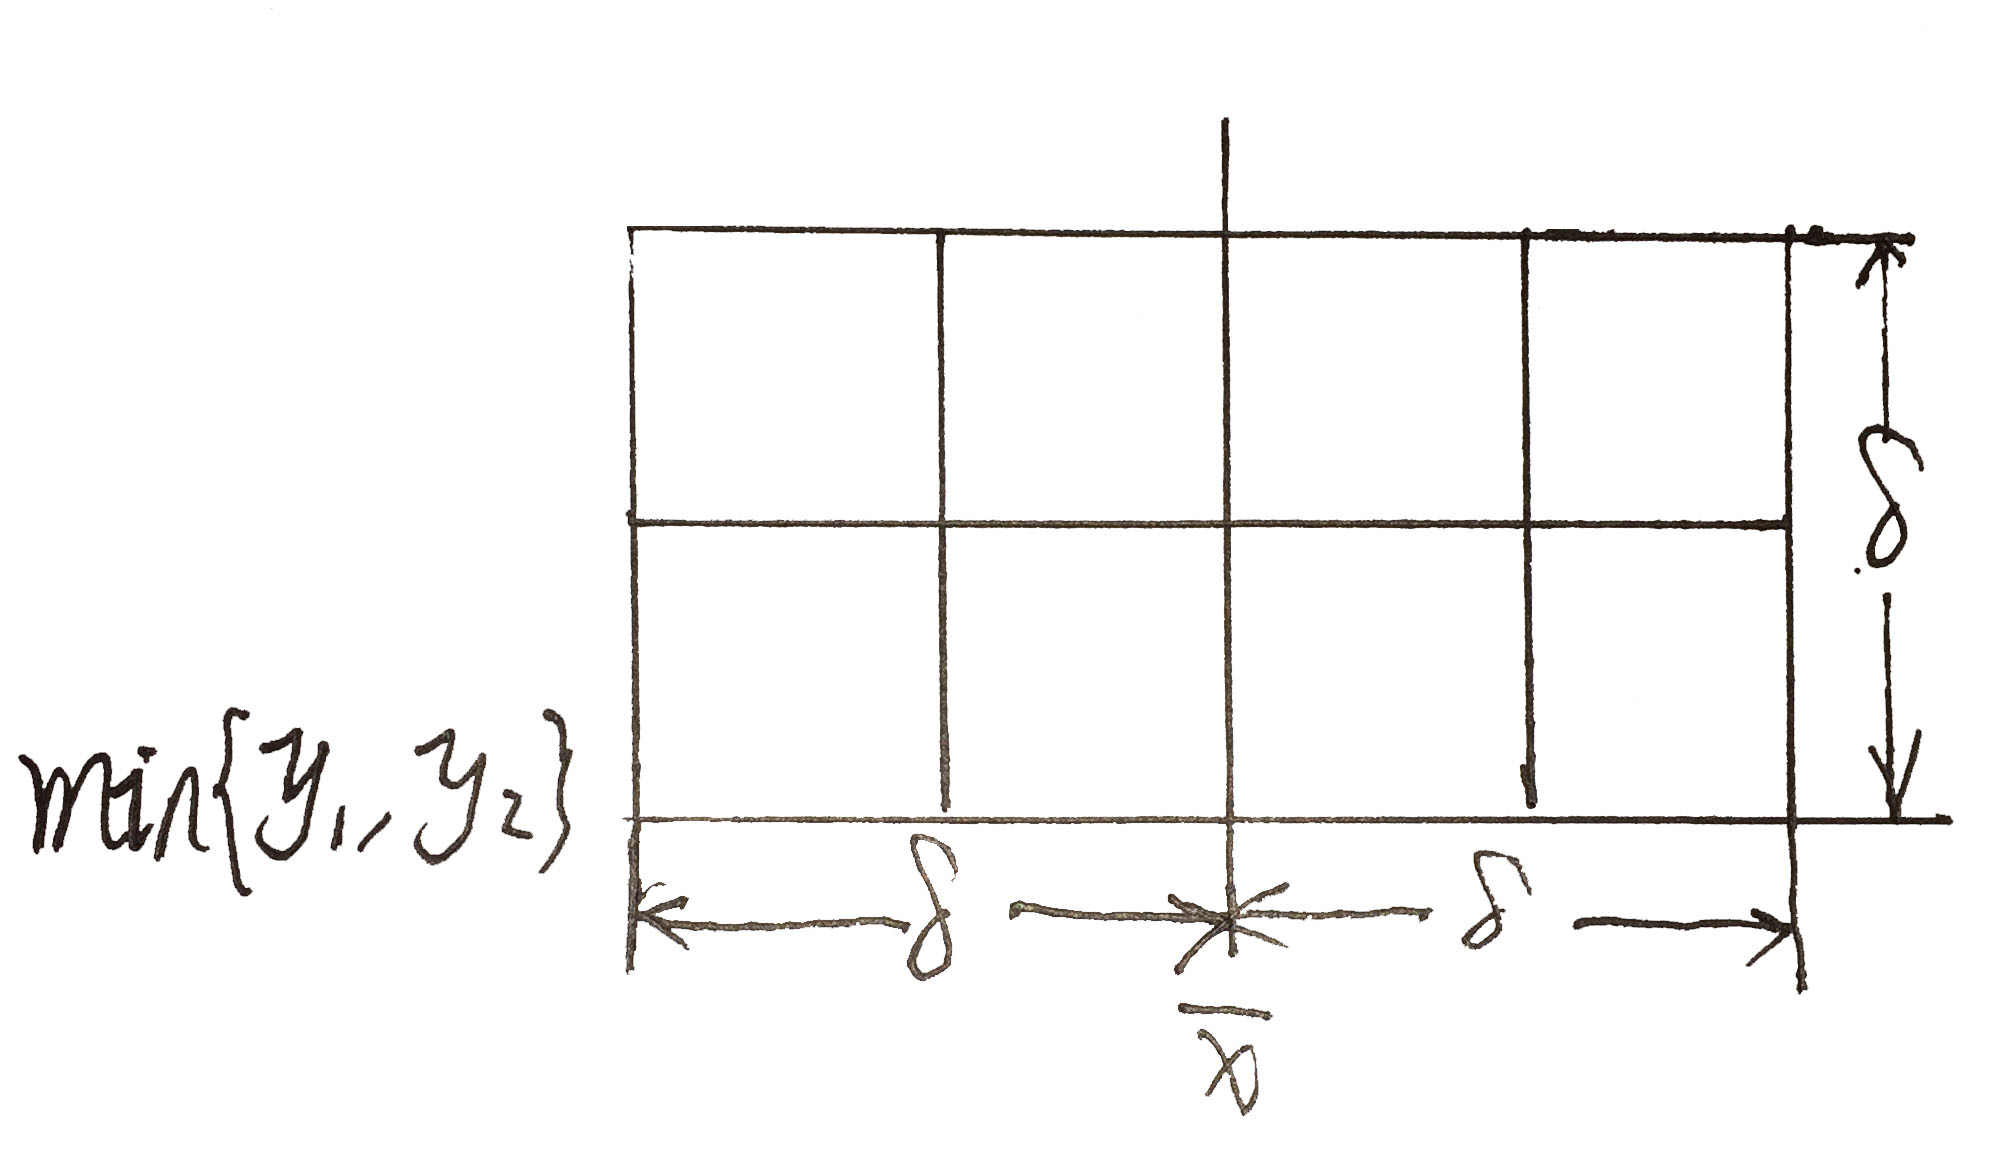
\includegraphics[width=0.5\textwidth]{closestpointlemma.jpg}
\caption{$p,q$ at most 7 positions away from each other}\label{pq7position}
\end{figure}

In Figure \ref{pq7position}, we draw 8 $\delta/2\times\delta/2$ grids around $\overline{x}$ and $\min\{y_1,y_2\}$. Since $\lvert y_1-y_2\rvert<d(p,q)<\delta$ and $p,q\in S_y$, we know that $p,q$ must be contained in these grids. On the other hand, each grid can contain at most 1 point, because if a grid contained 2 points, their distance would be smaller than $\sqrt{2}/2\delta$, thus smaller than $\delta$, violating the prerequisite that $\delta$ is the minimum distance between a non-split pair. As a result, there can be at most 8 points inside these grids, including $p$ and $q$. Hence $p,q$ are at most 7 points away from each other.
\end{proof}
According to Lemma \ref{lemmaforclosesplitpair}, we finally have the \texttt{ClosestSplitPair} algorithm as shown in Algorithm \ref{closestsplitpair}.
\begin{algorithm}[ht]
\caption{ClosestSplitPair($P_x,P_y,\delta$)}\label{closestsplitpair}
\begin{algorithmic}[1]
\Input\Statex{$P_x,P_y,\delta$ as defined in Algorithm \ref{closetpair}.}
\Output\Statex{Split pair $p\in Q,q\in R$ with $d(p,q)<\delta$, or $null$ if such pair does not exist.}
\State{Initialize $best = \delta$, $best\_pair=null$}
\For{$i$ = 1 \textbf{to} $\lvert S_y\rvert-1$}
\For{$j$ = 1 \textbf{to} $\min\{7,\lvert S_y\rvert-i\}$}
\State{Let $p,q$ be $i^{th}$, $(i+j)^{th}$ points of $S_y$}
\If{$d(p,q)<best$}
\State{$best\_pair = p,q,\:best=d(p,q)$}
\EndIf
\EndFor
\EndFor
\end{algorithmic}
\end{algorithm}
\section{The Master Method}
Potentially useful algorithmic ideas often need mathematical analysis to evaluate. The master method is a general recurrence approach to analyze the running time of divide-and-conquer algorithms. 
\subsection{Examples}
Recall the integer multiplication problem. Let $T(n)$ represent the maximum number of primitive operations needed to multiply two $n$-digit integers. The recurrence approach aims at expressing $T(n)$ in terms of running time of recursive calls concerning smaller $n$. In this specific divide-and-conquer algorithm, we hope to express $T(n)$ as function of $T(n/2)$. A recurrence approach needs a base case. In this problem the base case is trivial: $T(1)\leq a$, in which $a$ is a constant.

For the divide-and-conquer algorithm without Gauss's trick, we have 
\begin{equation}\label{nogausstrick}
T(n)\leq 4\cdot T(n/2)+O(n).
\end{equation}
When Gauss's trick is applied, we have 
\begin{equation}\label{gausstrick}
T(n)=3\cdot T(n/2)+O(n).
\end{equation}
Merge sort takes $O(n\log n)$ running time. It has the recurrence relation
\begin{equation}\label{mergesortrecur}
T(n)=2\cdot T(n/2)+O(n).
\end{equation}
We have no idea how to obtain the running time from these recurrence relations, but it is clear that the rank of the three algorithms in terms of running time is \eqref{nogausstrick}$>$\eqref{gausstrick}$>$\eqref{mergesortrecur}.
\subsection{Mathematical Statement}
The master method helps to obtain the running time of an algorithm according to its recurrence relation. It assumes that all sub-problems have equal size, thus it's not applicable to the closest pair problem, in which the left and right halves of the points are not guaranteed to have the same number of points. We also assume that the base case is trivial: $T(n)\leq a$ ($a$ is constant) for all sufficiently small $n$. Consider an algorithm that has the recurrence relation
\begin{equation*}
T(n)\leq a\cdot T(n/b)+O(n^d),
\end{equation*}
in which $a,b,n$ are constants with clear meanings. $a$ is the number of recursive calls, $b$ is the input size shrinkage factor, and $O(n^d)$ describes the amount of work needed to combine the solutions to the sub-problems. $a,b$ are both larger than 1, while $d$ can be as small as 0. Master method provides the form of $T(n)$ in different cases, as expressed in Theorem \ref{mastermethod}.
\begin{theorem}\label{mastermethod}
$T(n)$ can be expressed in big-O notation as follow\footnote{If the recurrence relation is written with = rather than $\leq$, the result will be in $\Theta$ notation.}:
\begin{equation*}
T(n)=
\begin{cases}
O(n^d\log n)&\text{if}\:a=b^d\\
O(n^d)&\text{if}\:a<b^d\\
O(n^{\log_ba})&\text{if}\:a>b^d\\
\end{cases}
\end{equation*}
\end{theorem}
Now let's look at a few examples. 

For merge sort algorithm \ref{mergesort} with recurrence relation \eqref{mergesortrecur}, we have $a=2,\:b=2,\:d=1$, thus it belongs to case 1 and has running time $O(n\log n)$. 

Consider binary search, which has the recurrence relation
\begin{equation*}
T(n)=T(n/2)+O(1),
\end{equation*} 
i.e. $a=1,\:b=2,\:d=0$, hence it is $O(\log n)$. 

For the integer multiplication algorithm without Gauss's trick \eqref{nogausstrick}, we have $a=4,\:b=2,\:d=1$, ending up with case 3. Thus it has time complexity $O(n^2)$, i.e. the divide-and-conquer approach fails to improve the time consumption in comparison with the primary school method. 

When we take Gauss's trick into account, i.e. with Karatsuba multiplication algorithm \ref{kmultiplication}, in \eqref{gausstrick} we have $a=3,\:b=2,\:d=1$. We are still in case 3 and end up with $O(n^{\log_23})$, which is smaller than $O(n^2)$ but larger than $O(n\log n)$.

Strassen's algorithm \ref{strassen} for matrix multiplication has the recurrence relation
\begin{equation*}
T(n)=7\cdot T(n/2)+O(n^2),
\end{equation*}
which leaves us in case 3. Its running time is therefore $O(n^{\log_27})$, which is better than $O(n^3)$.

As an illustration of case 2, consider the recurrence relation 
\begin{equation*}
T(n)\leq 2\cdot T(n/2)+O(n^2).
\end{equation*}
With $a=b=d=2$, we are in case 2, and end up with running time $O(n^2)$. In this case, the running time is governed by the work outside the recursive call, i.e. the time spent on combining solutions to the sub-problems dominates the global time consumption.
\subsection{Proof}
We will prove the correctness of the master method in this section. As having been stated above, we assume that the recurrence relation takes the form
\begin{itemize}
\item $T(1)\leq c$
\item $T(n)\leq a\cdot T(n/b)+cn^d$
\end{itemize} 
It's fine to use the same constant $c$ in both the base case and the recurrence relation because we are using $\leq$. In order to make the process less tedious, we also assume that $n$ is a power of $b$. The argument will be similar to what we did to obtain the running time of merge sort: through analysis on the recursive tree. Note that in this section when we refer to a value of time consumption, we always mean that the actual time consumption is smaller than or equal to this value.

The recursive tree has $\log_bn+1$ levels, from level 0 (the original problem) to level $\log_bn$ (trivial problem of size 1). At level $j$, there are in total $a^j$ sub-problems, each of size $n/b^j$. For $j\neq\log_bn$, the time consumption at this level is contributed by the $cn^d$ term:
\begin{equation*}
a^j\cdot c\cdot\left(\frac{n}{b^j}\right)^d=c\cdot n^d\cdot\left(\frac{a}{b^d}\right)^j.
\end{equation*}
Summing it up over all levels leads to the result $c\cdot n^d\cdot\sum\limits_{j=0}^{\log_bn-1}\left(\frac{a}{b^d}\right)^j$. At level $\log_bn$, the time consumption is simply the combination of all base cases:
\begin{equation*}
c\cdot a^{\log_bn}
\end{equation*}
The total time consumption is thus 
\begin{equation}\label{totaltime}
c\cdot n^d\cdot\sum\limits_{j=0}^{\log_bn-1}\left(\frac{a}{b^d}\right)^j+c\cdot a^{\log_bn}=c\cdot n^d\cdot\sum\limits_{j=0}^{\log_bn}\left(\frac{a}{b^d}\right)^j
\end{equation}
This leads to classified discussion over the value of $\frac{a}{b^d}$.
\begin{enumerate}
\item $a=b^d$. In this case, \eqref{totaltime} becomes 
\begin{equation*}
c\cdot n^d(\log_bn+1)=O(n^d\log_bn)
\end{equation*}
\item $a<b^d$. In this case, \eqref{totaltime} becomes 
\begin{equation*}
c\cdot n^d\frac{1-\left(\frac{a}{b^d}\right)^{\log_bn+1}}{1-\frac{a}{b^d}}<\frac{c}{1-\frac{a}{b^d}}n^d=O(n^d)
\end{equation*}
\item $a>b^d$. In this case, \eqref{totaltime} becomes 
\begin{equation*}
c\cdot n^d\frac{\left(\frac{a}{b^d}\right)^{\log_bn+1}-1}{\frac{a}{b^d}-1}<\frac{c}{\frac{a}{b^d}-1}n^d\frac{a}{b^d}\left(\frac{a}{b^d}\right)^{\log_bn}=O(a^{\log_bn})=O(n^{\log_ba})
\end{equation*}
\end{enumerate}
Therefore we have completed the proof of the master method.\hfill$\square$

The essential role that $a/b^d$ plays here comes naturally from the meaning of $a,b,d$. Each problem produces $a$ sub-problems in the next level. We call $a$ the \textbf{rate of sub-problem proliferation, abbr. RSP}. Size of each sub-problem shrinks by $b$ times after each recurrence, and the work load shrinks by $b^d$ times, so we call $b^d$ the \textbf{rate of work shrinkage, abbr. RWS}. The three cases of the master method can be interpreted as follow.
\begin{enumerate}
\item RSP = RWS. The amount of work at each level is $cn^d$. With totally $\log_bn$ levels, the problem should be $O(n^d\log_bn)$.
\item RSP $>$ RWS. The amount of work increases with the recursion level $j$. The last level dominates the running time, thus the overall running time is proportional to the number of sub-problems (base cases) in the last level. The problem is $O(a^{\log_bn})$.
\item RSP $<$ RWS. The amount of work decreases with the recursion level $j$. The root level dominates the running time, thus the problem is $O(n^d)$. 
\end{enumerate}
\ifx\PREAMBLE\undefined
\end{document}
\fi